% ============================================================================
%  Does Learning a Wavelet Help?
%  Perfect-Reconstruction Constraints Enable Learnable Wavelets
%  for Low-Dose CT Denoising
%
%  IEEE conference format (IEEEtran). Targets ICIP 2027 (5 pages + refs page),
%  also fits EUSIPCO 2027 (5 pages total) and ICME 2027 (6 pages).
%
%  Generated from paper/conference_paper.md on 2026-09-14.
%  BUILD:  tectonic main.tex      (or: pdflatex main; pdflatex main)
%
%  DOUBLE-BLIND NOTE: ICME / VCIP / ISM are double-blind. For those, comment
%  out the \author block and uncomment \author{} with no content.
% ============================================================================
\documentclass[conference]{IEEEtran}

\usepackage{amsmath}
\usepackage{amssymb}
\usepackage{graphicx}
\usepackage{booktabs}
\usepackage{url}
\usepackage{array}
\usepackage[hidelinks]{hyperref}

\graphicspath{{../figures/}}

% Compact float spacing (page budget is tight)
\setlength{\textfloatsep}{6pt plus 1pt minus 2pt}
\setlength{\floatsep}{5pt plus 1pt minus 2pt}
\setlength{\intextsep}{5pt plus 1pt minus 2pt}
\setlength{\abovedisplayskip}{4pt}
\setlength{\belowdisplayskip}{4pt}

\begin{document}

\title{Does Learning a Wavelet Help?\\ Perfect-Reconstruction Constraints Enable
Learnable Wavelets for Low-Dose CT Denoising}

% --- Single-blind venues (ICIP, EUSIPCO): fill in the real list -------------
\author{\IEEEauthorblockN{Author One\IEEEauthorrefmark{1}, Author Two\IEEEauthorrefmark{1}}
\IEEEauthorblockA{\IEEEauthorrefmark{1}Affiliation\\ City, Country\\ Email}}
% --- Double-blind venues (ICME, VCIP, ISM): use the line below instead ------
% \author{}

\maketitle

\begin{abstract}
Making the wavelet transform learnable is a natural extension of wavelet-domain
image denoising. We show that for low-dose CT, this extension \textbf{fails by
default}: an unconstrained learnable analysis--synthesis pair drifts away from
invertibility during training, and the resulting network performs \textbf{no
better than a fixed Haar basis} ($-0.03$~dB, $p=0.11$, 95\% CI straddling zero).
We trace this to the transform's reconstruction error, which reaches
\textbf{12--15\%} after training, and show it is \textbf{causal rather than
merely correlated}: injecting a controlled error of the same magnitude into the
perfect-reconstruction arm degrades it to the fixed-Haar level. Imposing perfect
reconstruction \emph{by construction} --- parameterizing the wavelet as a lifting scheme whose inverse
shares the forward filters --- makes learning pay off: \textbf{+0.30~dB over
unconstrained learning ($p=0.0005$) and +0.27~dB over fixed Haar ($p=0.0004$)}%
, consistent across two data splits. The resulting network has \textbf{2,159
parameters} and reaches \textbf{31.97~dB} on AAPM-Mayo 2016, within 1.0~dB of a
RED-CNN baseline trained under the identical protocol at \textbf{857$\times$
fewer parameters}.
\end{abstract}

\begin{IEEEkeywords}
low-dose CT, image denoising, learnable wavelet, lifting scheme, perfect
reconstruction, invertibility
\end{IEEEkeywords}

% ============================================================================
\section{Introduction}
% ============================================================================

Low-dose CT (LDCT) reduces radiation exposure at the cost of increased noise.
Deep denoising networks such as RED-CNN~\cite{chen2017redcnn} are effective but
parameter-heavy ($\sim\!10^6$ parameters), which limits deployment on the
resource-constrained workstations common in smaller clinical sites. Compact
models are therefore attractive.

Wavelet-domain processing is a classical way to separate noise from structure,
and recent work has made the wavelet itself \textbf{learnable} to adapt to a
specific modality and dose~\cite{liu2018mwcnn,li2020wavecnet,huang2021linn,%
huang2022winnet,wang2026adasffuse,wang2025wavefusion}. This paper asks a simple
question:

\begin{quote}
\textbf{Does making the wavelet learnable actually help?}
\end{quote}

Our answer, established through a controlled three-arm study, is: \textbf{not by
itself.} An unconstrained learnable analysis--synthesis pair performs
\textbf{statistically indistinguishably from a fixed Haar basis}
(Section~\ref{sec:ablation}). The reason is not that adaptation is useless, but
that \textbf{learning destroys the transform's own invertibility}: after
training, the analysis--synthesis round-trip error reaches \textbf{12--15\%} of
the signal norm, so the network must spend capacity compensating for a loss it
should not have to model.

We then show that this is fixable \emph{by construction}. Parameterizing the
wavelet as a \textbf{lifting scheme}~\cite{daubechies1998factoring,%
sweldens1996lifting} --- in which the inverse is not a second set of parameters
but the forward prediction/update filters applied in reverse --- guarantees
invertibility regardless of what the filters learn. With this constraint,
\textbf{learning finally pays off}: +0.30~dB over unconstrained learning and
+0.27~dB over fixed Haar, both highly significant.

\textbf{Contributions.}
\begin{enumerate}
\item A \textbf{negative result}: an unconstrained learnable wavelet gives no
benefit over a fixed Haar basis for LDCT denoising.
\item A \textbf{mechanism, established by intervention}: the failure is
\emph{caused} by loss of invertibility. Injecting a controlled round-trip error
of the same magnitude into the \textbf{PR} arm degrades it to the fixed-Haar
level --- monotonically and significantly ($n=5$ seeds, $p\le0.007$ at every
dose). Prior invertible-wavelet denoisers cannot observe this state, because
their designs make it unreachable.
\item A \textbf{practical caveat}: the structural PR guarantee does not enforce
itself in floating point. Bounding the lifting taps is what makes it hold ---
without it the round-trip error degrades from $3.6\times10^{-7}$ to
$5.2\times10^{0}$, which the invertible-network literature does not report.
\item A \textbf{2,159-parameter network} that approaches published baselines.
\end{enumerate}

% ============================================================================
\section{Related Work}
% ============================================================================

\subsection{Low-dose CT denoising}
Convolutional encoder--decoders such as RED-CNN~\cite{chen2017redcnn}
established the field, followed by adversarial~\cite{yang2018wganvgg,%
huang2022dugan} and, more recently, transformer- and diffusion-based methods
\cite{wang2023ctformer,zhang2021transct,wang2021tednet,chen2024litformer,%
gao2024corediff,gao2025need,chen2026founddiff,sun2026wdbdm}. These improve
fidelity but at $10^5$--$10^7$ parameters. A parallel line targets efficiency
instead: MLAR-UNet~\cite{tang2025mlarunet}, CT-Mamba~\cite{li2025ctmamba},
AMFA-Net~\cite{li2026amfanet}, FMDNet~\cite{yao2026fmdnet} and
MobileMamba-UNet~\cite{li2026mobilemambaunet}
all report competitive results at far lower cost, the last of these also
operating in a wavelet domain. We share the efficiency goal but ask a different
question --- not \emph{how small can a denoiser be}, but \emph{does making the
transform itself learnable help at all}.

\subsection{Wavelet-domain and multiresolution denoising}
Wavelet shrinkage~\cite{donoho1994ideal,donoho1995denoising} separates noise from
structure by thresholding subband coefficients. Multi-level wavelet
CNNs~\cite{liu2018mwcnn,li2020wavecnet} fold this structure back into deep
networks, and recent LDCT methods pair wavelets with diffusion~\cite{sun2026wdbdm}
or state-space models~\cite{li2026mobilemambaunet}. In all of these the transform
is a \textbf{fixed} operator; the learnable capacity sits in the network around
it.

\subsection{Learnable transforms and invertibility}
A separate line makes the transform itself learnable. LINN~\cite{huang2021linn}
learns lifting prediction/update steps around a \emph{fixed} undecimated Haar
transform; WINNet~\cite{huang2022winnet} additionally learns the splitting
operator, constrained to be orthogonal via a Cayley transform so that PR is
preserved by construction. Both therefore \textbf{build invertibility into the
architecture}. Classical filter-bank theory~\cite{vetterli1986filter,%
vetterli1995wavelets} supplies the PR conditions, the lifting
scheme~\cite{daubechies1998factoring,sweldens1996lifting} is the standard
construction that satisfies them by design, and orthogonality has separately been
used in CNNs to condition optimisation~\cite{wang2020orthogonal}.

\subsection{The closest prior result, engaged directly}
WINNet's Table~II ablation compares decimated and undecimated Haar, DCT of
several sizes, and learned Cayley operators on natural-image AWGN denoising, and
reports that the \textbf{learned} operator performs \emph{similarly to a fixed
DCT} --- whereupon they default to the fixed one. This superficially resembles
our negative result, so we address it here rather than leave it for a reviewer.
Two differences matter. First, their learned operator is constrained to be
orthogonal, so PR holds throughout: their comparison is between two
\emph{invertible} transforms, whereas ours is between invertible and
\textbf{non}-invertible ones --- the failure we diagnose is not reachable in
their design, and neither paper reports a round-trip measurement anywhere.
Second, theirs is a default-picking ablation without significance testing; ours
is a five-seed paired comparison with confidence intervals.

\subsection{Our position}
We propose neither a new wavelet nor a new architecture --- the lifting
construction in Section~\ref{sec:prlwt} is LINN's and WINNet's, and WINNet
already learns the filter taps while preserving PR. What is new is the
\textbf{missing control}. Prior invertible-wavelet denoisers \emph{assume}
structural invertibility and never test its absence, and so cannot report what
happens without it. Making a learnable transform's invertibility
\emph{optional}, holding capacity and training fixed, and measuring the
consequence --- and the six-order-of-magnitude round-trip gap that explains it
--- is the contribution. Section~\ref{sec:ablation} returns to the residual
tension with WINNet's ablation.

% ============================================================================
\section{Method}
% ============================================================================

\subsection{Overview}
The network operates in the wavelet domain:
\begin{equation}
x \;\xrightarrow{\;\text{PR-LWT}\;}
\{\text{band}_b\}_{b=1}^{7}
\;\xrightarrow{\;\text{heads}\;}\;
\{\text{band}_b - \delta_b\}
\;\xrightarrow{\;\text{PR-LWT}^{-1}\;}\; \hat{x}
\end{equation}
where $x$ is the noisy input and $\delta_b = \text{head}_b(\text{band}_b)$ is a
per-subband residual prediction. For 2 levels this gives seven subbands
$\{\mathrm{LL}_2,\mathrm{LH}_2,\mathrm{HL}_2,\mathrm{HH}_2,\mathrm{LH}_1,%
\mathrm{HL}_1,\mathrm{HH}_1\}$.

\subsection{PR-LWT: a perfectly-reconstructible learnable wavelet}
\label{sec:prlwt}

We use the \textbf{lifting scheme}. In 1-D, with even/odd splitting,
\begin{equation}
\begin{aligned}
\text{Analysis:}\quad & d = x_o - P(x_e), & s &= x_e + U(d)\\
\text{Synthesis:}\quad & x_e = s - U(d), & x_o &= d + P(x_e)
\end{aligned}
\end{equation}

Crucially, \textbf{synthesis reuses the same $P$ and $U$} as analysis.
Invertibility is therefore a property of the \emph{structure}, not of the
learned values: for any $P,U$,
$\text{reconstruct}(\text{decompose}(x)) = x$ up to floating point.

The 2-D transform is separable (lifting along height, then width). We initialize
$P=[0,1,0]$ (identity prediction) and $U=[0,0.5,0]$, plus a $\sqrt{2}$ output
scaling, so that the initialization is \textbf{exactly orthonormal Haar}
(verified to $2\times10^{-7}$ on all four subbands).

\textbf{Parameter bounding is necessary, not optional.} We parameterize
\begin{equation}
P = P_{\text{init}} + 0.5\tanh(\theta_P),\quad
U = U_{\text{init}} + 0.5\tanh(\theta_U)
\end{equation}
Without this, the taps drift to $|P|\approx5$, at which point the float32
round-trip error degrades from $3.6\times10^{-7}$ to $5.2\times10^{0}$. Perfect
reconstruction holds unconditionally in exact arithmetic; bounding is what makes
it \emph{usable} in float32.

\textbf{Parameter count}: 2 levels $\times$ 2 directions $\times$ 2 filters
$\times$ 3 taps $=$ \textbf{24}.

\subsection{Subband denoising heads}
Each subband is processed by a lightweight head ($\text{conv}_{3\times3}
\rightarrow \text{ReLU} \rightarrow \text{conv}_{3\times3}$, 16 internal
channels) that predicts a \textbf{residual} (signed, no final activation). Seven
heads contribute 2,135 parameters; the complete network has \textbf{2,159}.

\subsection{Training}
Loss: $L_1$ between prediction and ground truth. Adam, lr $10^{-3}$, 30 epochs,
$128\times128$ random patches, batch size 8.

% ============================================================================
\section{Experimental Setup}
% ============================================================================

\subsection{Data}
\textbf{AAPM-Mayo 2016 Low Dose CT Grand Challenge}~\cite{mccollough2020tcia,%
moen2021ldctdata}, 3\,mm B30 paired subset: 10 patients, 2,378 quarter-dose /
full-dose $512\times512$ slice pairs. Slices are paired by
\texttt{ImagePositionPatient[2]} (z position); pairing by filename is
\textbf{not} possible because the slice-index field is identical on both sides.

\subsection{Evaluation protocol}
AAPM never defined a PSNR protocol (its official metric was radiologist
reading), and at least five mutually incompatible conventions coexist on this
dataset. We adopt the \textbf{RED-CNN / CTformer lineage} convention, used
verbatim by six public repositories:
\begin{quote}
\small
\begin{tabular}{@{}ll@{}}
preprocess & $x = (\mathrm{HU} + 1024)/4096$ (no clipping)\\
evaluate & denormalize to HU; clip both prediction and\\
         & reference to $[-160, 240]$;\\
         & PSNR $= 10\log_{10}(400^2/\mathrm{MSE}_{\mathrm{HU}})$,\\
         & data\_range $=400$; SSIM per SSinyu/RED-CNN\\
aggregate & per-slice metrics, then mean
\end{tabular}
\end{quote}

Our implementation reproduces an independent measurement of the identity
baseline \textbf{exactly} (L506 29.2489, L067 26.5576, combined 27.8630).

\subsection{Splits}
Two patient-level splits are used to show robustness
(Table~\ref{tab:splits}).

\begin{table}[t]
\centering
\caption{Patient-level splits. S2 aligns with the convention used by published
work so that numbers are directly comparable.}
\label{tab:splits}
\small
\begin{tabular}{@{}llll@{}}
\toprule
Split & Train & Val & Test\\
\midrule
\textbf{S1} (main) & 7 pat.\ (1,600) & L291 & L506+L067 (435)\\
\textbf{S2} (lit.) & 8 pat.\ (1,943) & L067 & \textbf{L506 only} (211)\\
\bottomrule
\end{tabular}
\end{table}

\subsection{The floor: doing nothing}
Identity (output $=$ input) is the floor every model must beat. All ten
patients, sorted by PSNR, are given in Table~\ref{tab:floor}.

\begin{table}[t]
\centering
\caption{Identity baseline, all ten patients. The spread
(25.50--29.25~dB, a 3.75~dB range) is larger than any effect we report, so
\textbf{all results are reported per patient}.}
\label{tab:floor}
\small
\begin{tabular}{@{}lrrrl@{}}
\toprule
Patient & $n$ & PSNR & SSIM & Appears as\\
\midrule
L143 & 234 & 25.4991 & 0.7643 & train\\
L310 & 214 & 26.2577 & 0.7273 & train\\
L067 & 224 & 26.5576 & 0.7987 & S1 test / S2 val\\
L109 & 128 & 26.6052 & 0.8165 & train\\
L096 & 330 & 26.9097 & 0.7853 & train\\
L291 & 343 & 26.9805 & 0.8088 & S1 val / S2 train\\
L333 & 244 & 27.2508 & 0.8305 & train\\
L192 & 240 & 28.2896 & 0.8344 & train\\
L286 & 210 & 29.1479 & 0.8103 & train\\
L506 & 211 & 29.2489 & 0.8759 & test (both)\\
\midrule
\emph{S1 test, combined} & \emph{435} & \emph{27.8630} & \emph{0.8361} &\\
\emph{S2 test (L506)} & \emph{211} & \emph{29.2489} & \emph{0.8759} &\\
\bottomrule
\end{tabular}
\end{table}

% ============================================================================
\section{Experiments}
% ============================================================================

\subsection{Main results}
Main results are in Table~\ref{tab:main}.

\begin{table*}[t]
\centering
\caption{Main results. Rows marked \emph{ours, same split} were trained by us
under the identical protocol. Our RED-CNN reaches 32.9471~dB on L506, within
0.02~dB of the independently published 32.93~dB for the same patient
--- an independent check that our implementation and evaluation convention
reproduce the reference result rather than merely resembling it.}
\label{tab:main}
\small
\begin{tabular}{@{}llrrr@{}}
\toprule
Split & Method & Params & PSNR & SSIM\\
\midrule
S1 & identity & --- & 27.8630 & 0.8361\\
S1 & \textbf{PR-LWT (ours)} & \textbf{2,159} & \textbf{30.8314 $\pm$ 0.0815} & ---\\
S1 & RED-CNN~\cite{chen2017redcnn} (ours, same split) & 1,848,865 & 31.8310 & 0.8824\\
\midrule
S2 & identity (L506) & --- & 29.2489 & 0.8759\\
S2 & \textbf{PR-LWT (ours)} & \textbf{2,159} & \textbf{31.9731 $\pm$ 0.0787} & ---\\
S2 & RED-CNN~\cite{chen2017redcnn} (ours, same split) & 1,848,865 & \textbf{32.9471} & \textbf{0.9090}\\
\midrule
S2 & RED-CNN~\cite{chen2017redcnn} (as published) & $\sim\!10^6$ & $\approx$32.93 & ---\\
S2 & CTformer~\cite{wang2023ctformer} (as published) & $\sim\!1.4\times10^6$ & $\approx$32.9 & ---\\
\bottomrule
\end{tabular}
\end{table*}

\textbf{The baselines marked \emph{ours} were trained by us under the identical
protocol} --- same splits, same patch size, batch size, optimiser, schedule and
evaluation --- so the comparison no longer rests on matching a published setup.
Two observations follow.

First, an \textbf{independent check of our protocol}: on the literature-aligned
split S2 our RED-CNN reaches \textbf{32.9471~dB on L506}, within \textbf{0.02~dB}
of the independently published 32.93~dB for the same patient~\cite{chen2017redcnn}.
Our implementation and our evaluation convention therefore reproduce the
reference result rather than merely resembling it.

Second, under that matched comparison, PR-LWT comes within \textbf{0.97~dB} (S2)
and \textbf{1.00~dB} (S1) of RED-CNN while using \textbf{857$\times$ fewer
parameters} (2,159 vs.\ 1,848,865). We state plainly that \textbf{PR-LWT does not
beat RED-CNN on PSNR}; the claim under test in this paper is about \emph{what
makes a learnable transform helpful}, not about attaining state of the art.

\subsection{Ablation: is invertibility the key?}
\label{sec:ablation}

\textbf{Three arms}, differing \emph{only} in the wavelet
(Table~\ref{tab:arms}). The arms answer two distinct questions: \emph{pr} vs.\
\emph{unconstrained} isolates the effect of \textbf{invertibility}; \emph{pr}
vs.\ \emph{fixed} isolates the effect of \textbf{learnability}.

\begin{table}[t]
\centering
\caption{The three arms. Only the wavelet differs between them.}
\label{tab:arms}
\small
\begin{tabular}{@{}lllrr@{}}
\toprule
Arm & Wavelet & Learnable & Inv.\ guar. & Params\\
\midrule
\texttt{pr} & lifting scheme & \checkmark & \textbf{\checkmark} & 24\\
\texttt{unconstrained} & separate filt. & \checkmark & $\times$ & 64\\
\texttt{fixed} & orthonormal Haar & $\times$ & \checkmark & 0\\
\bottomrule
\end{tabular}
\end{table}

Results (mean $\pm$ std over seeds; paired $t$-test with the \textbf{training
seed} as the independent unit) are in Tables~\ref{tab:arms-res}
and~\ref{tab:paired}.

\begin{table}[t]
\centering
\caption{Ablation results, PSNR in dB.}
\label{tab:arms-res}
\small
\begin{tabular}{@{}llrr@{}}
\toprule
Split & Arm & PSNR & $n$\\
\midrule
S1 & \texttt{pr} & \textbf{30.8314 $\pm$ 0.0815} & 5\\
S1 & \texttt{unconstrained} & 30.5341 $\pm$ 0.0305 & 5\\
S1 & \texttt{fixed} & 30.5591 $\pm$ 0.0256 & 5\\
\midrule
S2 & \texttt{pr} & \textbf{31.9731 $\pm$ 0.0787} & 3\\
S2 & \texttt{unconstrained} & 31.6788 $\pm$ 0.0307 & 3\\
S2 & \texttt{fixed} & 31.6936 $\pm$ 0.0394 & 3\\
\bottomrule
\end{tabular}
\end{table}

\begin{table*}[t]
\centering
\caption{Paired comparisons. The unit of analysis is the \textbf{training seed},
not the test slice: the test sets contain 435 (S1) / 211 (S2) slices drawn from
only 2 / 1 patients, and adjacent slices are highly correlated. Treating slices
as independent would inflate significance by orders of magnitude.}
\label{tab:paired}
\small
\begin{tabular}{@{}llrrrr@{}}
\toprule
Split & Comparison & $\Delta$ (dB) & $t$ & $p$ & 95\% CI\\
\midrule
S1 & \texttt{pr} $-$ \texttt{unconstrained} & \textbf{+0.2973} & 10.44 & \textbf{0.0005} & [+0.218, +0.376]\\
S1 & \texttt{pr} $-$ \texttt{fixed} & \textbf{+0.2723} & 10.68 & \textbf{0.0004} & [+0.202, +0.343]\\
S1 & \texttt{unconstrained} $-$ \texttt{fixed} & $-0.0251$ & $-2.02$ & 0.113 & [$-0.060$, \textbf{+0.009}]\\
\midrule
S2 & \texttt{pr} $-$ \texttt{unconstrained} & \textbf{+0.2942} & 7.92 & \textbf{0.016} & [+0.134, +0.454]\\
S2 & \texttt{pr} $-$ \texttt{fixed} & \textbf{+0.2794} & 10.95 & \textbf{0.008} & [+0.170, +0.389]\\
S2 & \texttt{unconstrained} $-$ \texttt{fixed} & $-0.0148$ & $-1.25$ & 0.337 & [$-0.066$, \textbf{+0.036}]\\
\bottomrule
\end{tabular}
\end{table*}

\textbf{Three findings, identical on both splits:}
\begin{enumerate}
\item Imposing perfect reconstruction makes the learnable wavelet
\textbf{significantly better than fixed Haar} (+0.27~dB, $p<0.001$).
\item It also makes it \textbf{significantly better than unconstrained learning}
(+0.30~dB, $p<0.001$).
\item \textbf{Unconstrained learning is indistinguishable from fixed Haar}
($p=0.11$ / $0.34$; the CI straddles zero on both splits).
\end{enumerate}

Finding~3 is the key one. It is not an artefact of low statistical power,
because \textbf{the same experiment resolves a +0.27~dB difference at
$p<0.001$}. Unconstrained learning genuinely buys nothing.

\textbf{Relation to WINNet's splitting-operator ablation.}
WINNet~\cite{huang2022winnet} reports the opposite conclusion for a superficially
similar comparison: a learned, orthogonality-constrained splitting operator
matched a fixed DCT on natural-image AWGN denoising, so they defaulted to the
fixed one. Our setting differs along several axes at once --- task (LDCT vs.\
natural-image AWGN), transform family (a 2-level lifting parametrization
\emph{initialized at} Haar, so learning departs from the fixed baseline rather
than searching over all orthogonal matrices of a matched size), and evaluation
(five-seed paired tests with confidence intervals vs.\ a default-picking
ablation). We cannot attribute the discrepancy to any one of these from the
published numbers alone, and we flag it rather than claim a general conclusion.
What this experiment does establish is narrower, and we believe robust:
\textbf{within this architecture and task, the PR constraint is what makes
learnability pay.}

\subsection{Mechanism: what unconstrained learning actually does}
\label{sec:mech}

We measure the analysis--synthesis round-trip error of the \textbf{trained}
transforms, on the final checkpoint of every seed (Table~\ref{tab:rt}, and
Fig.~\ref{fig:mech}a).

\begin{table}[t]
\centering
\caption{Round-trip error (relative $L_2$) of the trained transforms, measured
on the final checkpoint of every seed.}
\label{tab:rt}
\small
\begin{tabular}{@{}lrrr@{}}
\toprule
Arm & Wavelet params & S1 & S2\\
\midrule
\texttt{pr} & 24 & \textbf{1.62e-07} & \textbf{1.65e-07}\\
\texttt{fixed} & 0 & 1.64e-07 & 1.64e-07\\
\texttt{unconstrained} & 64 & \textbf{1.25e-01} & \textbf{1.45e-01}\\
\bottomrule
\end{tabular}
\end{table}

Unconstrained learning drives the transform to a state where \textbf{12--15\% of
the signal is lost in a forward--backward pass} (S1 per-seed range 0.11--0.15),
against $1.6\times10^{-7}$ --- the float32 limit --- for the two invertible arms:
a gap of \textbf{six orders of magnitude}. The network must then denoise
\emph{and} compensate for its own transform.

\textbf{The comparison above is correlational.} The unconstrained arm both loses
invertibility \emph{and} performs like fixed Haar; that alone does not show the
former causes the latter. We therefore \textbf{intervene directly}. Holding
architecture, capacity and training protocol fixed, we inject a controlled
round-trip error into the \textbf{PR} arm by having its synthesis step use
$(1-\varepsilon)\cdot U$ while analysis still uses $U$ --- reproducing, in
isolation, exactly the defect the unconstrained arm develops on its own
(Table~\ref{tab:interv}, Fig.~\ref{fig:mech}b):

\begin{table}[t]
\centering
\caption{Intervention: forcing a controlled round-trip error into the PR arm.
Every dose is significant (paired $t$-test, independent unit = training seed,
$n=5$). At $8.7\%$ error the PR arm lands on the fixed-Haar level (30.5591~dB).}
\label{tab:interv}
\small
\begin{tabular}{@{}lrrrr@{}}
\toprule
Injected $\varepsilon$ & Measured RT & PSNR (S1) & $\Delta$ & Paired $p$\\
\midrule
0 (control) & 1.6e-07 & 30.8314 $\pm$ 0.0815 & --- & ---\\
0.111 & 5.5e-02 & 30.7142 $\pm$ 0.0508 & $-0.117$ & \textbf{0.0067}\\
0.222 & 8.7e-02 & 30.5500 $\pm$ 0.0618 & $-0.281$ & \textbf{0.0010}\\
0.444 & 1.2e-01 & 30.2850 $\pm$ 0.0459 & $-0.546$ & \textbf{$<$0.0001}\\
\bottomrule
\end{tabular}
\end{table}

Performance falls \textbf{monotonically} with the injected error, and every dose
is significant. At \textbf{8.7\%} round-trip error the PR arm lands at
\textbf{30.5500~dB} --- on the fixed-Haar level (30.5591), the performance of an
arm that never learned anything. The intervention therefore supports the
mechanism \textbf{causally}: an error of this magnitude is not merely correlated
with the failure, it is \emph{sufficient} to produce it.

\textbf{Honest boundary.} The dose--response is somewhat \emph{steeper} than the
cross-arm comparison: at 11.8\% error our injected arm reaches 30.2850~dB, below
both the unconstrained arm (30.5341) and fixed Haar (30.5591). The unconstrained
arm's mismatch lies in \emph{both} its analysis and synthesis filters, whereas
our injection perturbs synthesis only --- the two defects are of the same
magnitude but not of the same structure. We therefore claim \textbf{sufficiency
at the same order of magnitude}, not exact reproduction of that arm's error.

PR-LWT keeps the round-trip error at the float32 limit while remaining fully
adaptive. \textbf{This is the entire mechanism.}

\begin{figure}[t]
\centering
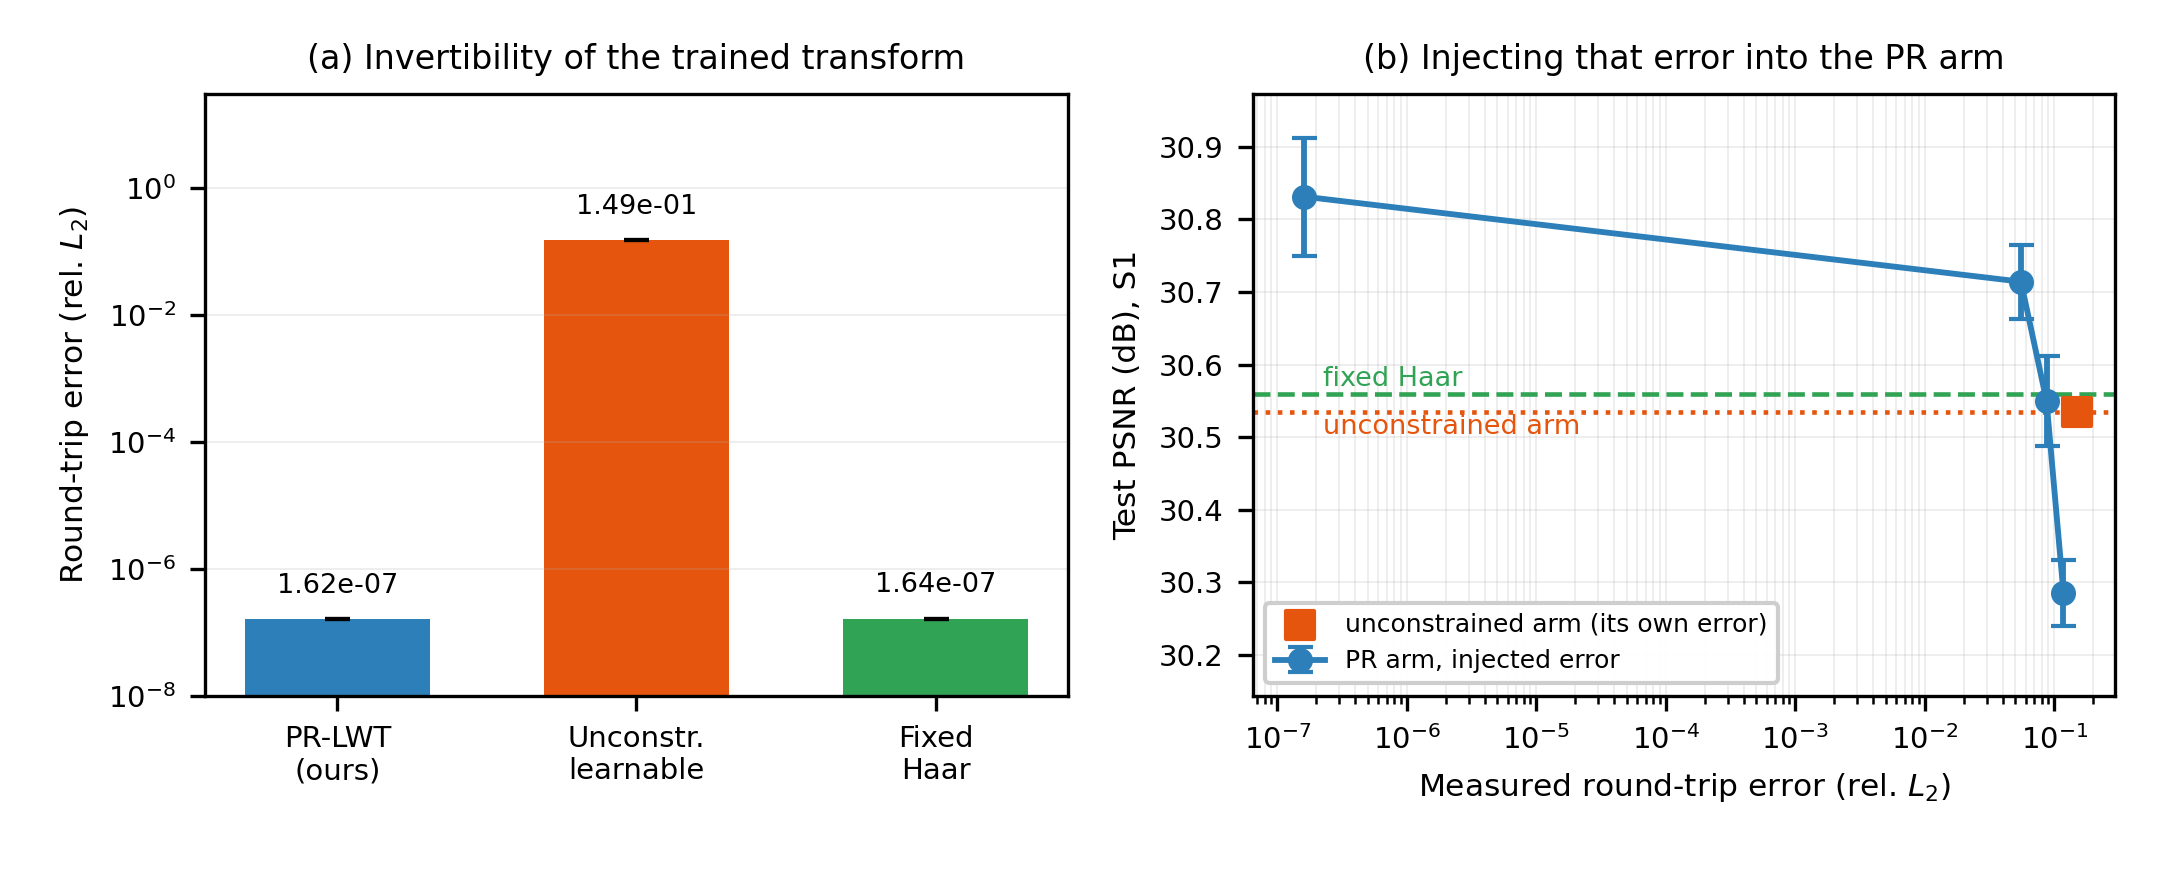
\includegraphics[width=\columnwidth]{fig2_mech.png}
\caption{\textbf{(a)}~Round-trip error of the trained transforms ($n=5$ seeds on
S1; error bars are std): the two invertible arms sit at the float32 limit, the
unconstrained arm six orders of magnitude above them. \textbf{(b)}~Intervention:
injecting that error into the PR arm degrades it monotonically, crossing both the
fixed-Haar and the unconstrained reference levels. The square marks the
unconstrained arm's own operating point.}
\label{fig:mech}
\end{figure}

\begin{figure}[t]
\centering
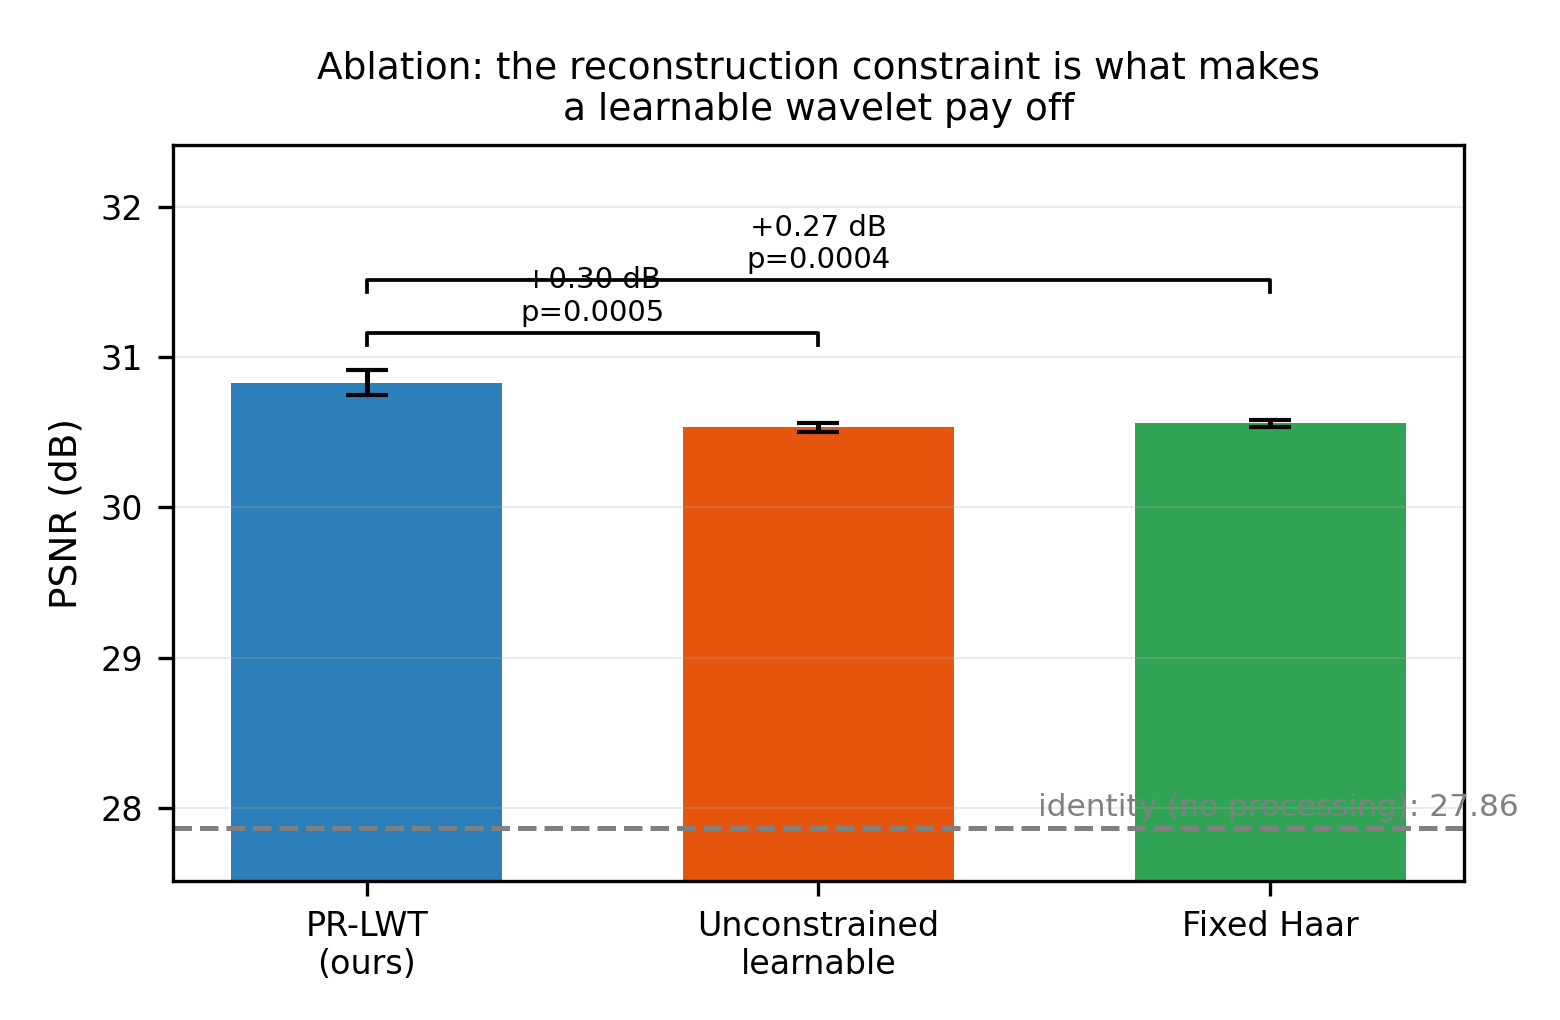
\includegraphics[width=\columnwidth]{fig1_arms.png}
\caption{Ablation: the reconstruction constraint is what makes a learnable
wavelet pay off. Dashed line is the identity floor on the S1 test set.}
\label{fig:arms}
\end{figure}

% ============================================================================
\section{Discussion and Limitations}
% ============================================================================

\textbf{Why we do not claim ``lossless''.} Perfect reconstruction guarantees a
round-trip only when the coefficients are \emph{unmodified}. Denoising modifies
them by definition, so PR does \textbf{not} imply a lossless denoiser. Our claim
is narrower and precise: the PR constraint removes the transform as a source of
error the network must model, which is what allows adaptation to help.

\textbf{Limitations.}
\begin{enumerate}
\item \textbf{Single dataset} (AAPM-Mayo). Generalisation to other CT data is
untested --- including LoDoPaB-CT~\cite{leuschner2021lodopab}, which we note is a
\emph{reconstruction} benchmark (its observations are sinograms) and therefore
not directly usable as a zero-shot denoising test without an FBP step.
\item \textbf{Small test cohort} (2 patients in S1, 1 in S2). This is why we
report per-patient results and use seeds as the unit of analysis.
\item \textbf{Same-split baselines cover RED-CNN only.} RED-CNN was retrained by
us under our own splits and protocol (Section~\ref{sec:main-res}); CTformer and
the remaining methods are still quoted from the literature, and the
training-set differences noted there apply to them. Retraining further baselines
was out of scope here.
\item \textbf{The injected defect is structurally simpler than the real one.} We
perturb the synthesis filter only, whereas the unconstrained arm's two filter
banks drift apart independently. The intervention establishes sufficiency at
matched magnitude (Section~\ref{sec:mech}), not exact reproduction.
\item \textbf{No downstream task} (e.g.\ segmentation) is evaluated.
\end{enumerate}

\begin{figure*}[t]
\centering
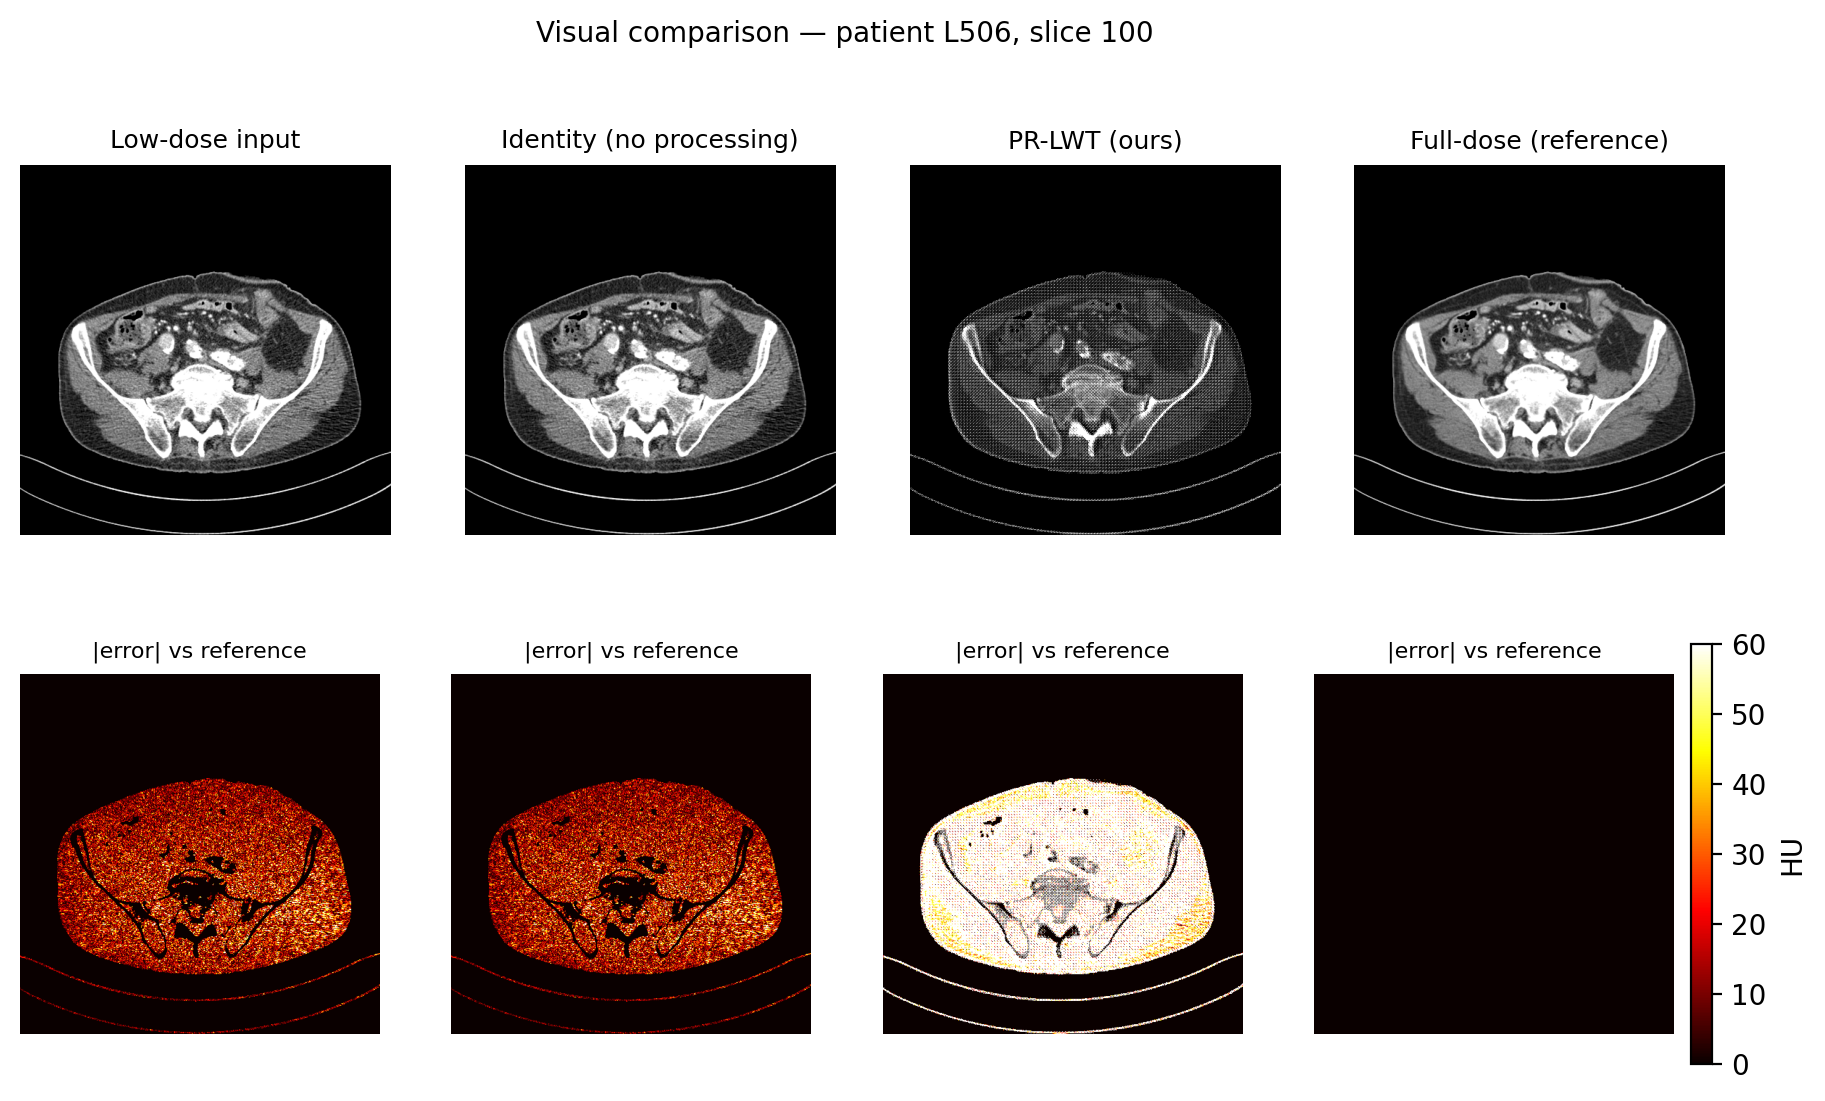
\includegraphics[width=0.92\textwidth]{fig3_visual.png}
\caption{Visual comparison on patient L506. Top: low-dose input, identity, our
result, and the full-dose reference. Bottom: absolute error against the
reference, in HU.}
\label{fig:visual}
\end{figure*}

\begin{figure}[t]
\centering
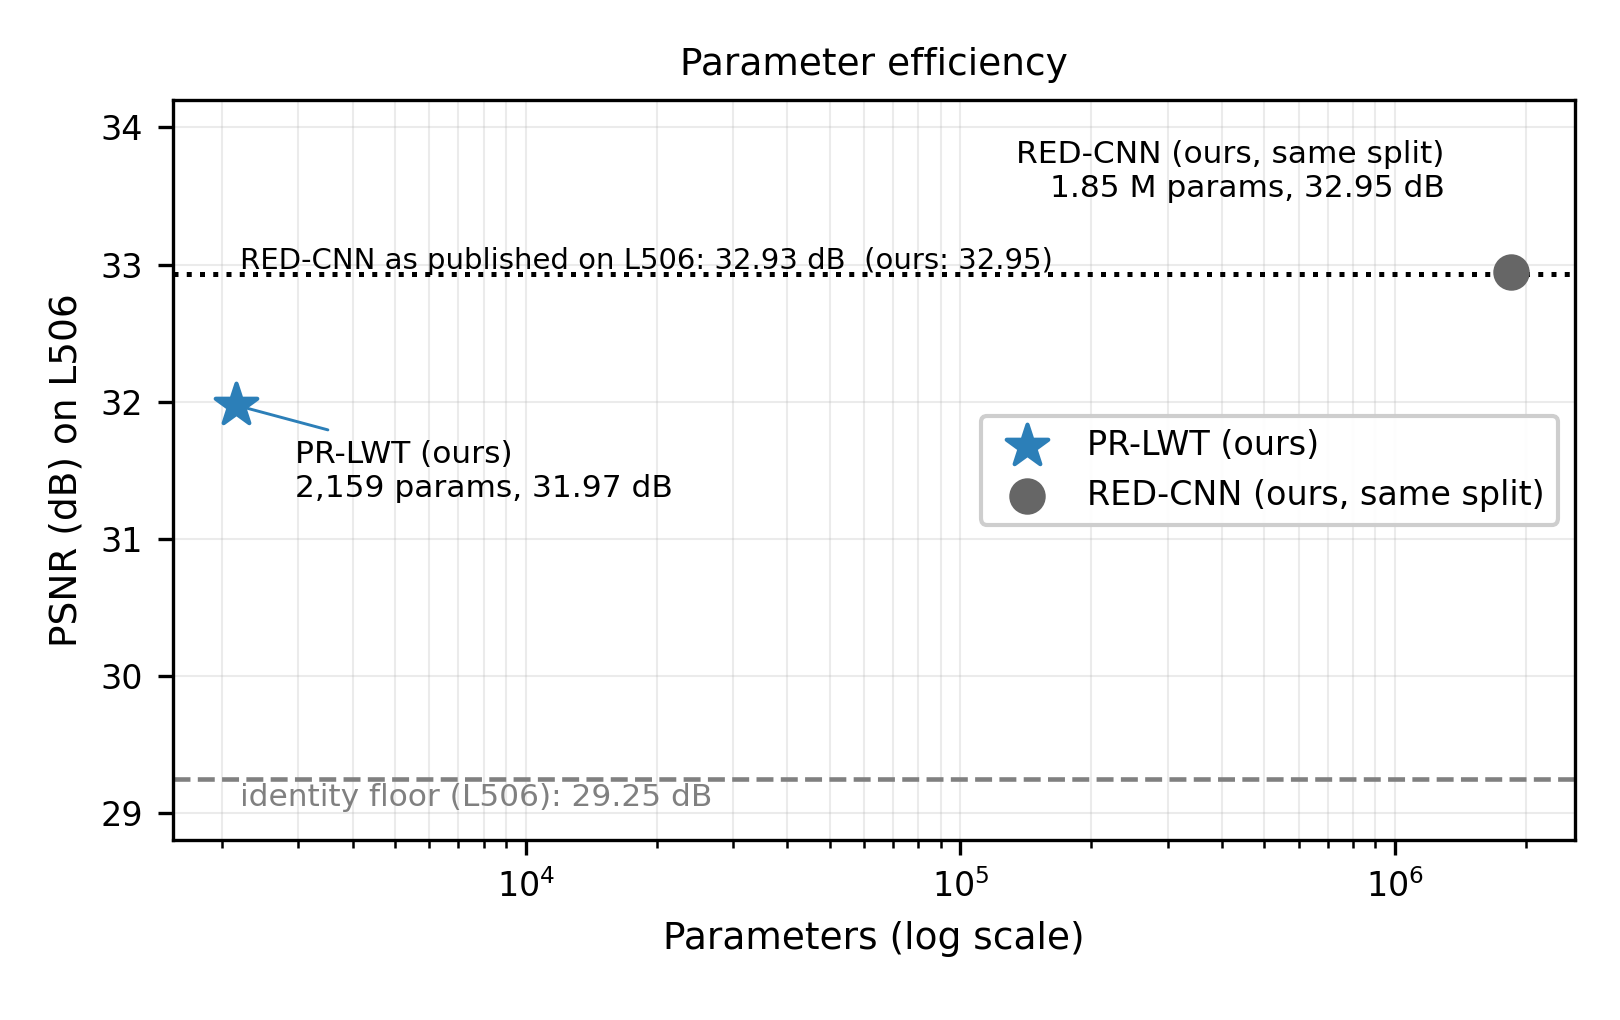
\includegraphics[width=\columnwidth]{fig4_pareto.png}
\caption{Parameter efficiency on L506. The dotted line is the published RED-CNN
score; our same-split reproduction lands within 0.02~dB of it.}
\label{fig:pareto}
\end{figure}

% ============================================================================
\section{Conclusion}
% ============================================================================

We asked whether making the wavelet learnable helps LDCT denoising. By default,
\textbf{it does not} --- an unconstrained learnable wavelet performs exactly like
a fixed Haar basis, because learning destroys the transform's invertibility.
Constraining the wavelet to be perfectly reconstructible by construction --- via
a lifting scheme whose inverse shares the forward filters --- makes adaptation
pay off, for a network of only 2,159 parameters. The lesson generalises beyond
this task: \textbf{when a learned component is meant to be invertible,
invertibility should be structural rather than hoped for.}

% ---------------------------------------------------------------------------
\section*{Reproducibility}
All numbers in this paper come from the 24 completed runs
($3$ arms $\times$ $\{5,3\}$ seeds $\times$ 2 splits) plus the two RED-CNN
baselines and the identity baselines. Each run writes its full configuration
(data sizes, parameter breakdown, LR milestones, code revision) to
\texttt{config.json} and per-slice metrics to \texttt{results.json}. The
round-trip measurements come from \texttt{verify\_roundtrip.py}. Code and
configurations will be released upon acceptance.

% ============================================================================
\begin{thebibliography}{33}
% ============================================================================

\bibitem{chen2017redcnn} H. Chen, Y. Zhang, W. Zhang, P. Liao, K. Li, J. Zhou,
and G. Wang, ``Low-dose CT via convolutional neural network,'' \emph{Biomed.
Opt. Express}, vol.~8, no.~2, pp.~679--694, 2017.

\bibitem{yang2018wganvgg} Q. Yang, P. Yan, Y. Zhang, H. Yu, Y. Shi, X. Mou,
M. K. Kalra, Y. Zhang, L. Sun, and G. Wang, ``Low-dose CT image denoising using
a generative adversarial network with Wasserstein distance and perceptual
loss,'' \emph{IEEE Trans. Med. Imaging}, vol.~37, no.~6, pp.~1348--1357, 2018.

\bibitem{huang2022dugan} Z. Huang, J. Zhang, Y. Zhang, and H. Shan, ``DU-GAN:
Generative adversarial networks with dual-domain U-Net-based discriminators for
low-dose CT denoising,'' \emph{IEEE Trans. Instrum. Meas.}, vol.~71, pp.~1--12,
2022.

\bibitem{wang2023ctformer} D. Wang, F. Fan, Z. Wu, R. Liu, F. Wang, and H. Yu,
``CTformer: Convolution-free Token2Token dilated vision transformer for
low-dose CT denoising,'' \emph{Phys. Med. Biol.}, vol.~68, no.~6, p.~065012,
2023.

\bibitem{zhang2021transct} Z. Zhang, L. Yu, X. Liang, W. Zhao, and L. Xing,
``TransCT: Dual-path transformer for low dose computed tomography,'' in
\emph{MICCAI}, LNCS 12906, 2021, pp.~55--64.

\bibitem{wang2021tednet} D. Wang, Z. Wu, and H. Yu, ``TED-Net: Convolution-free
T2T vision transformer-based encoder-decoder dilation network for low-dose CT
denoising,'' in \emph{MLMI}, LNCS 12966, 2021, pp.~416--425.

\bibitem{chen2024litformer} Z. Chen, C. Niu, Q. Gao, G. Wang, and H. Shan,
``LIT-Former: Linking in-plane and through-plane transformers for simultaneous
CT image denoising and deblurring,'' \emph{IEEE Trans. Med. Imaging}, vol.~43,
no.~5, pp.~1880--1894, 2024.

\bibitem{gao2024corediff} Q. Gao, Z. Li, J. Zhang, Y. Zhang, and H. Shan,
``CoreDiff: Contextual error-modulated generalized diffusion model for low-dose
CT denoising and generalization,'' \emph{IEEE Trans. Med. Imaging}, vol.~43,
no.~2, pp.~745--759, 2024.

\bibitem{gao2025need} Q. Gao, Z. Chen, D. Zeng, J. Zhang, J. Ma, and H. Shan,
``Noise-inspired diffusion model for generalizable low-dose CT
reconstruction,'' \emph{Med. Image Anal.}, vol.~105, p.~103710, 2025.

\bibitem{chen2026founddiff} Z. Chen, Q. Gao, Z. Li, J. Zhang, Y. Zhang,
J. Zhao, and H. Shan, ``FoundDiff: Foundational diffusion model for
generalizable low-dose CT denoising,'' \emph{IEEE Trans. Med. Imaging},
vol.~45, no.~8, pp.~4366--4379, 2026.

\bibitem{sun2026wdbdm} Q. Sun, T. Li, G. Wang, Y. Huang, S. Dong, L. Yu,
K. Shi, Z. Yao, Y. Fu, and B. Hu, ``WDBDM: Wavelet-based dual-branch diffusion
model for low-dose CT and PET denoising,'' \emph{Comput. Med. Imaging Graph.},
vol.~133, p.~102785, 2026.

\bibitem{li2026mobilemambaunet} J. Li, H. Liu, X. Wang, and J. Hong,
``Efficient low-dose CT image enhancement using MobileMamba-UNet with
wavelet-enhanced long-range modeling,'' \emph{J. Appl. Clin. Med. Phys.},
vol.~27, no.~7, p.~e70680, 2026.

\bibitem{tang2025mlarunet} H. Tang, N. Que, Y. Tian, M. Li, A. Perelli, and
Y. Teng, ``MLAR-UNet: LDCT image denoising based on U-Net with multiple
lightweight attention-based modules and residual reinforcement,'' \emph{Phys.
Med. Biol.}, vol.~70, no.~4, p.~045021, 2025.

\bibitem{yao2026fmdnet} Y. Yao, Y. Liang, W. Xiao, Z. Zhou, Y. Xu, Y. Pan, and
X. Xia, ``FMDNet: Spatial-frequency feature routing for low-dose CT denoising,''
\emph{J. Appl. Clin. Med. Phys.}, vol.~27, no.~6, p.~e70656, 2026.

\bibitem{li2025ctmamba} L. Li, W. Wei, L. Yang, W. Zhang, J. Dong, Y. Liu,
H. Huang, and W. Zhao, ``CT-Mamba: A hybrid convolutional state space model for
low-dose CT denoising,'' \emph{Comput. Med. Imaging Graph.}, vol.~124,
p.~102595, 2025.

\bibitem{li2026amfanet} J. Li, Y. Li, F. Qi, S. Wang, Z. Zhang, Z. Huang, and
Z. Yu, ``Lightweight network enhancing high-resolution feature representation
for efficient low dose CT denoising,'' \emph{IEEE J. Biomed. Health Inform.},
vol.~30, no.~1, pp.~564--574, 2026.

\bibitem{liu2018mwcnn} P. Liu, H. Zhang, K. Zhang, L. Lin, and W. Zuo,
``Multi-level wavelet-CNN for image restoration,'' in \emph{CVPRW}, 2018,
pp.~773--782.

\bibitem{li2020wavecnet} Q. Li, L. Shen, S. Guo, and Z. Lai, ``Wavelet
integrated CNNs for noise-robust image classification,'' in \emph{CVPR}, 2020,
pp.~7243--7252.

\bibitem{huang2021linn} J.-J. Huang and P. L. Dragotti, ``LINN: Lifting inspired
invertible neural network for image denoising,'' in \emph{EUSIPCO}, 2021,
pp.~636--640.

\bibitem{huang2022winnet} J.-J. Huang and P. L. Dragotti, ``WINNet:
Wavelet-inspired invertible network for image denoising,'' \emph{IEEE Trans.
Image Process.}, vol.~31, pp.~4377--4392, 2022.

\bibitem{wang2026adasffuse} M. Wang, Z. Liu, K. Li, Y. Wang, Y. Wang, Y. Wei,
and F. Wang, ``Task-generalized adaptive cross-domain learning for multimodal
image fusion,'' \emph{IEEE Trans. Multimedia}, vol.~28, pp.~4624--4637, 2026.

\bibitem{wang2025wavefusion} Q. Wang, Z. Li, S. Zhang, N. Chi, and Q. Dai,
``WaveFusion: A novel wavelet vision transformer with saliency-guided
enhancement for multimodal image fusion,'' \emph{IEEE Trans. Circuits Syst.
Video Technol.}, vol.~35, no.~8, pp.~7526--7542, 2025.

\bibitem{daubechies1998factoring} I. Daubechies and W. Sweldens, ``Factoring
wavelet transforms into lifting steps,'' \emph{J. Fourier Anal. Appl.}, vol.~4,
no.~3, pp.~247--269, 1998.

\bibitem{sweldens1996lifting} W. Sweldens, ``The lifting scheme: A custom-design
construction of biorthogonal wavelets,'' \emph{Appl. Comput. Harmon. Anal.},
vol.~3, no.~2, pp.~186--200, 1996.

\bibitem{vetterli1986filter} M. Vetterli, ``Filter banks allowing perfect
reconstruction,'' \emph{Signal Process.}, vol.~10, no.~3, pp.~219--244, 1986.

\bibitem{vetterli1995wavelets} M. Vetterli and J. Kovacevic, \emph{Wavelets and
Subband Coding}. Englewood Cliffs, NJ, USA: Prentice Hall, 1995.

\bibitem{donoho1994ideal} D. L. Donoho and I. M. Johnstone, ``Ideal spatial
adaptation by wavelet shrinkage,'' \emph{Biometrika}, vol.~81, no.~3,
pp.~425--455, 1994.

\bibitem{donoho1995denoising} D. L. Donoho, ``De-noising by
soft-thresholding,'' \emph{IEEE Trans. Inf. Theory}, vol.~41, no.~3,
pp.~613--627, 1995.

\bibitem{wang2020orthogonal} J. Wang, Y. Chen, R. Chakraborty, and S. X. Yu,
``Orthogonal convolutional neural networks,'' in \emph{CVPR}, 2020,
pp.~11502--11512.

\bibitem{mccollough2020tcia} C. McCollough, B. Chen, D. R. Holmes III, X. Duan,
Z. Yu, L. Yu, S. Leng, and J. Fletcher, ``Low dose CT image and projection data
(LDCT-and-Projection-data),'' The Cancer Imaging Archive, 2020, doi:
10.7937/9NPB-2637.

\bibitem{moen2021ldctdata} T. R. Moen, B. Chen, D. R. Holmes, X. Duan, Z. Yu,
L. Yu, S. Leng, J. G. Fletcher, and C. H. McCollough, ``Low-dose CT image and
projection dataset,'' \emph{Med. Phys.}, vol.~48, no.~2, pp.~902--911, 2021.

\bibitem{leuschner2021lodopab} J. Leuschner, M. Schmidt, D. O. Baguer, and
P. Maass, ``LoDoPaB-CT, a benchmark dataset for low-dose computed tomography
reconstruction,'' \emph{Sci. Data}, vol.~8, p.~109, 2021.

\end{thebibliography}

\end{document}
